\documentclass[14pt]{extbook}
\usepackage{multicol, enumerate, enumitem, hyperref, color, soul, setspace, parskip, fancyhdr} %General Packages
\usepackage{amssymb, amsthm, amsmath, latexsym, units, mathtools} %Math Packages
\everymath{\displaystyle} %All math in Display Style
% Packages with additional options
\usepackage[headsep=0.5cm,headheight=12pt, left=1 in,right= 1 in,top= 1 in,bottom= 1 in]{geometry}
\usepackage[usenames,dvipsnames]{xcolor}
\usepackage{dashrule}  % Package to use the command below to create lines between items
\newcommand{\litem}[1]{\item#1\hspace*{-1cm}\rule{\textwidth}{0.4pt}}
\pagestyle{fancy}
\lhead{Module12M}
\chead{}
\rhead{Version C}
\lfoot{1000-6427}
\cfoot{}
\rfoot{test}
\begin{document}

\begin{enumerate}
\item{
} \newpage
\item{
Using the scenario below, model the situation using an exponential function and a base of $\frac{1}{2}$. Then, solve for the half-life of the element, rounding to the nearest day.
\begin{center}
    \textit{ The half-life of an element is the amount of time it takes for the element to decay to half of its initial starting amount. There is initially 974 grams of element $X$ and after 3 years there is 108 grams remaining. }
\end{center}
} \newpage
\item{
For the scenario below, use the model for the volume of a cylinder as $V = \pi r^2 h$.
\begin{center}
    \textit{ Pringles wants to add 43 \text{percent} more chips to their cylinder cans and minimize the design change of their cans. They've decided that the best way to minimize the design change is to increase the radius and height by the same percentage. What should this increase be? }
\end{center}
} \newpage
\item{
Determine the appropriate model for the graph of points below.
\begin{center}
    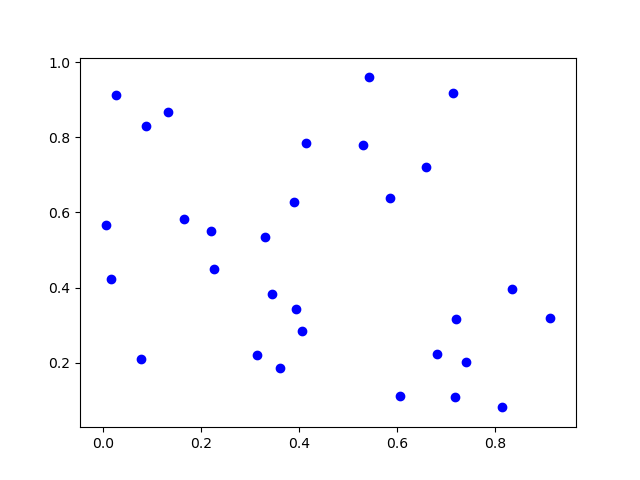
\includegraphics[width=0.5\textwidth]{../Figures/identifyModelGraph12CopyC.png}
\end{center}
} \newpage
\item{
For the scenario below, use the model for the volume of a cylinder as $V = \pi r^2 h$.
\begin{center}
    \textit{ Pringles wants to add 37 \text{percent} more chips to their cylinder cans and minimize the design change of their cans. They've decided that the best way to minimize the design change is to increase the radius and height by the same percentage. What should this increase be? }
\end{center}
} \newpage
\item{
Determine the appropriate model for the graph of points below.
\begin{center}
    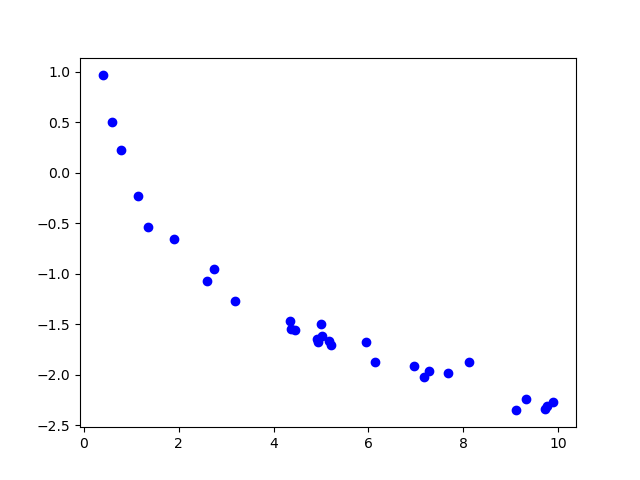
\includegraphics[width=0.5\textwidth]{../Figures/identifyModelGraph12C.png}
\end{center}
} \newpage
\item{
Solve the modeling problem below, if possible.
\begin{center}
    \textit{ In CHM2045L, Brittany created a 18 liter 25 percent solution of chemical $\chi$ using two different solution percentages of chemical $\chi$. When she went to write her lab report, she realized she forgot to write the amount of each solution she used! If she remembers she used 15 percent and 43 percent solutions, what was the amount she used of the 43 percent solution? }
\end{center}
} \newpage
\item{
Solve the modeling problem below, if possible.
\begin{center}
    \textit{ A new virus is spreading throughout the world. There were initially 8 many cases reported, but the number of confirmed cases has quadrupled every 5 days. How long will it be until there are at least 10000 confirmed cases? }
\end{center}
} \newpage
\item{
Solve the modeling problem below, if possible.
\begin{center}
    \textit{ In CHM2045L, Brittany created a 19 liter 19 percent solution of chemical $\chi$ using two different solution percentages of chemical $\chi$. When she went to write her lab report, she realized she forgot to write the amount of each solution she used! If she remembers she used 18 percent and 33 percent solutions, what was the amount she used of the 33 percent solution? }
\end{center}
} \newpage
\item{
Solve the modeling problem below, if possible.
\begin{center}
    \textit{ A new virus is spreading throughout the world. There were initially 5 many cases reported, but the number of confirmed cases has tripled every 2 days. How long will it be until there are at least 10000 confirmed cases? }
\end{center}
} \newpage
\end{enumerate}

\end{document}